\documentclass[psfig,preprint]{aastex}
                                                                                
\begin{document}
                                                                                
\title{SJU RADAR AT 1385 Mhz WITH DIFFERENT DIGITALMIX VALUES}

\author{Carl Heiles (\today)}

%\tableofcontents

\section{INTRODUCTION}

	We examined plots of spectra for individual {\it togs} fits
files, averged over all cal-off records in each fits file for our three
trial values for \verb$digitalmix$. We looked at
three such plots for each \verb$digitalmix$ value as a feeble attempt to
get a statistical sample. In fact, this is a tiny fraction of the
available data, as there are typically about 36 fits files on each
observing day. 

	So we examined plots for 9 such fits files, 3 for each value of
\verb$digitalmix$. For each set of 3 we picked a representative plot.
These are shown in the three figures: \begin{enumerate}
	\item Figure \ref{0905} is for 05 September 2005 and has
\verb$digitalmix = 26$.
	\item Figure \ref{0912} is for 12 September 2005 and has
\verb$digitalmix = 27$.
	\item Figure \ref{920} is for 20 September 2005 and has
\verb$digitalmix = 25$.
\end{enumerate}

	In figure \ref{0905}, we see the radar at $\sim 1421.5$ MHz, 
particularly in receiver 0 (the bottommost plot). In some receivers we 
see maybe more radar at $\sim 1422.5$ MHz. There are also some narrow
spikes, one at 1420.0 MHz (which appears in all plots) and a couple
below 1418 MHz.

	The other two figures exhibit no radar. They do show the narrow
spikes, however. In particular, figure \ref{920} has one very close to
the HI line. It seems a bit more serious thn the spikes in figure
\ref{0912}. 

	On the basis of this limited sample, I agree that we should stay
away \verb$digitalmix = 26$.  I think we are better off with
\verb$digitalmix = 27$ than \verb$digitalmix = 25$ because spikes are
less onerous.  In addition, \verb$digitalmix = 27$ puts the narrowband
spectrum more nearly in the center of the wideband one (note the
positions of the HI line on the left-hand wideband spectra). 

	We are now observing with \verb$digitalmix = 25$. I think we
should change to \verb$digitalmix = 27$. If you agree, then someone (not
me) is going to have to make this change in the observing file. 

\begin{figure}[!p]
\begin{center}
\includegraphics[width=6in]{quickplot_0905.togs.ps}   
\end{center}
\caption{Quickplot spectra for {\it togs} on 5 Sep 2005.\label{0905}}
\end{figure}

\begin{figure}[!p]
\begin{center}
\includegraphics[width=6in]{quickplot_0912.togs.ps}   
\end{center}
\caption{Quickplot spectra for {\it togs} on 12 Sep 2005.\label{0912}}
\end{figure}

\begin{figure}[!p]
\begin{center}
\includegraphics[width=6in]{quickplot_920.togs.ps}   
\end{center}
\caption{Quickplot spectra for {\it togs} on 20 Sep 2005.\label{920}}
\end{figure}

\acknowledgements

        This research was supported in part by NSF grant AST 04-06987    
and by the NAIC.



\end{document}
		
